% HEADER
\noindent
{\textbf{128}}\qquad{\sffamily\textbf{CHƯƠNG 2}}\quad{\sffamily Giới hạn và Đạo hàm}
\vspace{4mm}

% DẢI 1: NỘI DUNG ĐẦU TRANG (CỘT LỀ TRÁI ĐỂ TRỐNG, CỘT PHẢI CHỨA NỘI DUNG)
\noindent
\hspace*{56mm}%
\begin{minipage}{130mm}
  Ký hiệu $\infty$ không đại diện cho một con số. Mặc dù vậy, biểu thức $\lim\limits_{x \to \infty} f(x) = L$ thường được đọc là
  \begin{list}{}{%
    \setlength{\leftmargin}{1.5em}%
    \setlength{\topsep}{2.5pt}%
    \setlength{\partopsep}{0pt}%
    \setlength{\itemsep}{1.5pt}%
    \setlength{\parsep}{0pt}%
  }
    \item ``giới hạn của $f(x)$, khi $x$ tiến tới vô cùng, là $L$''
    \item[\hspace*{0.5em}hoặc] ``giới hạn của $f(x)$, khi $x$ trở nên vô cùng lớn, là $L$''
    \item[\hspace*{0.5em}hoặc] ``giới hạn của $f(x)$, khi $x$ tăng không giới hạn, là $L$''
  \end{list}

  \vspace{1.5mm}
  Ý nghĩa của các cụm từ này được đưa ra bởi Định nghĩa 1. Một định nghĩa chính xác hơn, tương tự như định nghĩa $\varepsilon, \delta$ ở Mục 2.4, được trình bày ở phần cuối của mục này.

  \vspace{1.5mm}
  Các minh họa hình học của Định nghĩa 1 được thể hiện trong Hình 2. Chú ý rằng có nhiều cách để đồ thị của $f$ tiếp cận đường thẳng $y = L$ (được gọi là một \textit{tiệm cận ngang}) khi ta nhìn sang phía xa bên phải của mỗi đồ thị.
\end{minipage}

\vspace{3.5mm}

% DẢI 2: HÌNH 2 TRẢI DÀI TOÀN TRANG (FULL WIDTH)
\noindent
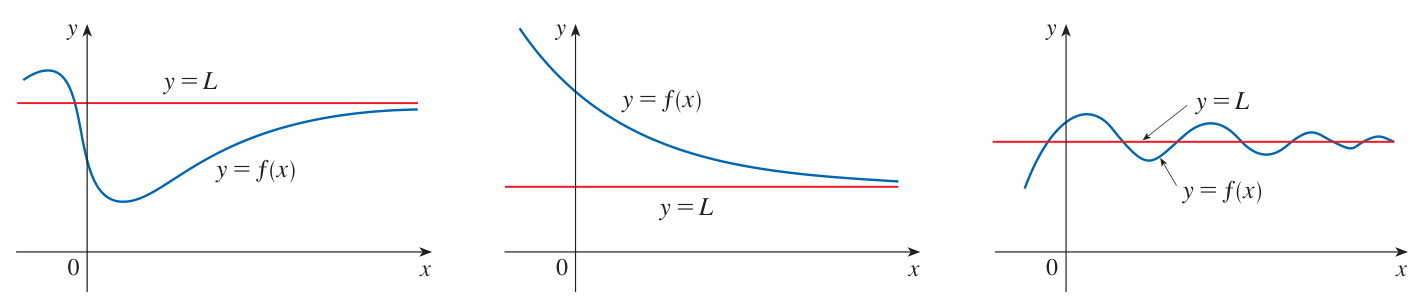
\includegraphics[width=\textwidth]{images/p0163_fig1.png}

\vspace{3.5mm}

% DẢI 3A: ĐOẠN DẪN VÀO ĐỊNH NGHĨA 2 (CỘT TRÁI ĐỂ TRỐNG DÓNG THEO LỀ HÌNH 2)
\noindent
\hspace*{56mm}%
\begin{minipage}{130mm}
  Nhìn lại Hình 1, ta thấy rằng đối với các giá trị âm có độ lớn lớn của $x$, các giá trị của $f(x)$ đều gần 1. Bằng cách cho $x$ giảm dần qua các giá trị âm không giới hạn, ta có thể làm cho $f(x)$ gần 1 tùy ý. Điều này được biểu diễn bằng cách viết
  \[
    \lim_{x \to -\infty} \frac{x^2 - 1}{x^2 + 1} = 1
  \]
  Định nghĩa tổng quát như sau.
\end{minipage}

\vspace{2.5mm}

% DẢI 3B: BỐ CỤC 2 CỘT (CỘT TRÁI CHỨA HÌNH 3, CỘT PHẢI CHỨA ĐỊNH NGHĨA 2 & 3)
\noindent
\begin{minipage}[t]{48mm}
  \vspace{0pt}
  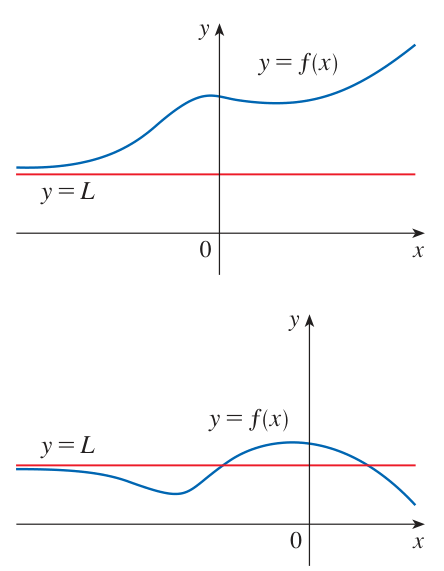
\includegraphics[width=\linewidth]{images/p0163_fig2.png}
\end{minipage}\hfill
\begin{minipage}[t]{130mm}
  \vspace{0pt}
  \begin{stewartdefbox}
    \defbadge{2}\enspace\textbf{\color{stewartred}Định nghĩa}\enspace Giả sử $f$ là một hàm số xác định trên một khoảng $(-\infty, a)$ nào đó. Khi đó
    \[
      \lim_{x \to -\infty} f(x) = L
    \]
    có nghĩa là các giá trị của $f(x)$ có thể làm gần $L$ tùy ý bằng cách lấy $x$ âm có giá trị tuyệt đối đủ lớn.
  \end{stewartdefbox}

  \vspace{2mm}
  Một lần nữa, ký hiệu $-\infty$ không biểu diễn một số, nhưng biểu thức $\lim\limits_{x \to -\infty} f(x) = L$ thường được đọc là
  \begin{center}
    \vspace{-1mm}
    ``giới hạn của $f(x)$, khi $x$ tiến tới âm vô cùng, là $L$''
    \vspace{-1mm}
  \end{center}

  Định nghĩa 2 được minh họa trong Hình 3. Chú ý rằng đồ thị tiếp cận đường thẳng $y = L$ khi ta nhìn sang phía xa bên trái của mỗi đồ thị.

  \vspace{2.5mm}
  \begin{stewartdefbox}
    \defbadge{3}\enspace\textbf{\color{stewartred}Định nghĩa}\enspace Đường thẳng $y = L$ được gọi là một \textbf{tiệm cận ngang} của đồ thị hàm số $y = f(x)$ nếu
    \[
      \lim_{x \to \infty} f(x) = L \qquad \text{hoặc} \qquad \lim_{x \to -\infty} f(x) = L
    \]
  \end{stewartdefbox}
\end{minipage}

% FOOTER BẢN QUYỀN
\vfill
\noindent
\begin{minipage}{\textwidth}
  \fontsize{5.5pt}{7pt}\selectfont\color{black!70}
  Bản quyền © 2021 Cengage Learning. Bảo lưu mọi quyền. Không được sao chép, quét hoặc nhân bản toàn bộ hay một phần. WCN 02-200-203\\[1pt]
  Do quyền kỹ thuật số, một số nội dung bên thứ ba có thể bị lược bỏ khỏi eBook và/hoặc eChapter. Đánh giá biên tập khẳng định mọi nội dung bị lược bỏ không ảnh hưởng đáng kể đến trải nghiệm học tập tổng thể. Cengage Learning bảo lưu quyền xóa nội dung bổ sung vào bất kỳ lúc nào nếu có yêu cầu hạn chế quyền tiếp theo.
\end{minipage}
